
% Introduction
In this chapter we will introduce the role of neuroergonomics in adaptive automation work environments and look at some of the problems that led to the current state of the field. 

\section{Introduction to the Field}
Neuroergonomics is often described as the study of brain and behavior at work. As the name suggests, neuroergonomics is comprised of two disciplines, neuroscience and ergonomics (also known as human factors). Neuroscience is concerned with the structure and the function of the brain. It is a highly interdisciplinary body of research spanning disciplines such as physiology, psychology, medicine, computer science, or mathematics. Human factors on the other hand is focused on examining the human use technology at work or other real-world settings. As the intersection of these two fields, neuroergonomics addresses both the brain and humans at work, but even more so their dynamic interaction \cite{Parasuraman2003}
. By understanding the neural bases of perceptual and cognitive functions, such as seeing, hearing, planing and decision making in relation to technology and settings in the real world, neuroergonomics strives to develop new optimization methods for various areas of applications. The additional value neuroergonomics can provide, compared to 'traditional' neuroscience and 'conventional' ergonomics, promises substantial economical benefits as well as significant improvements to health care and therefore society at large. 
In the scope of this thesis, we will focus primarily on applications in work settings such as modern automated systems. An area in which the effects of neuroergonomics are expected to be even greater, considering the difficulty of obtaining measures of overt behavior \cite{Parasuraman2003}.\\
Automated systems, in one form or another have been present in almost every branch of industry for the better part of what has been two centuries. Automation itself can be defined as the creation and application of technology by which the production and delivery of various goods and services is controlled and monitored with minimal human assistance. Automation can be encountered in many different places, from a simple control loop in a hydraulic system up to an artificial intelligence handling emergency breaking in autonomic cars.%, based on scans of the car's environment. 
Static automation is the original form of automation. In this form, automation is an all-or-none technology either performing a task for us or not \cite{Byrne2006}.
Although, there are numerous benefits (i.e. relieving workers from the strain of performing repetitive tasks) to it, there also is increasing evidence that static automation comes at the price of impaired decision making, manual skill degradation, loss of situational awareness, and monitoring inefficiency \cite{Byrne1996}.
These problems stem from the significant change of roles that automation causes in a work environment. What this means is that workers, once active operators of machines and technology, are now passive monitors who often face monitoring workloads that are inherently different and often significantly higher when compared to the manual control conditions of a non automated work environment. The continuous exposure to workloads that are either too high or too low can have dramatic effects on human-system performance, thereby potentially compromising safety \cite{Mehta2013}. This has already been indicated by the work of Parasuraman et al. (1993, 1994) who tested subjects in a multi-task flight simulator with optionally automatable components and reported a substantial decrease of human operator detection of automation failures after short periods of time in a static automation scenario with constant task assignment of both operator and the automated system \cite{Byrne1996}.
However, we must not forget the consequences these highly automated and ever so stressful workplaces have on human operators specifically. Studies by Cooper et al. showed that working in a stressful environment increases the risk of suffering physical illness or symptoms of psychological distress, as well as work related accidents and injuries \cite{Clarke2004}.\\
We will now take a look at what is called adaptive automation. Adaptive automation has been introduced to resolve the abovementioned issues of statically automated systems.
Whereas static automation is considered to be an agent working for the operator, adaptive automation is viewed as an interactive aid working with the operator \cite{Byrne1996}. It attempts to optimize system performance by adjusting the task assignment between the human operator and automation dynamically. This task reallocation is based on task demands, user capabilities, and system requirements. Meaning that during high task load conditions or emergencies the use of automation is increased and decreased during normal operations \cite{Mehta2013}.
Another advantage of adaptive over static automation is the ability to reconstruct the task environment in terms of what is automated, how it is automated, what tasks may be shared, and when changes occur \cite{Byrne1996}. 
However, for an adaptive system to be efficient we require both the operator and the automated system to have sufficient knowledge of each other's current capabilities, performance and state \cite{Byrne1996}.
As discussed by Byrne et al. (1996), there are three main approaches to address this issue, which either use model-based prediction or continuous measurements to determine the operators current state. In the scope of this thesis we will focus on the latter of the two. 
Usually, the way to measure human performance at work is to use physiological measures that reflect, more or less directly, aspects of brain functions. There is however a group of measures that is particularly favored among neuroergonomic researches. Those are the ones that are derived from the brain itself such as electroencephalography (\gls{eeg}), magnetencephalography (\gls{meg}), and event-related potentials (\gls{erp}), as well as measures related to the brain's metabolic and vascular responses such as positron emission tomography (\gls{pet}), and functional magnetic resonance imaging (\gls{fmri}) \cite{Parasuraman2003}. Although, there are many advantages to this group of measures, such as the temporal resolution of \gls{erp} and the spatial resolution of \gls{fmri}, there is still one major disadvantage. In fact, the majority of the abovementioned measures are either too expensive, impose too much restrictions on the movement of the subject, or are simply unfit to be used in a portable system, which ultimately prevents their application in real-world settings. Also, the lack of comfort and therefore low operator acceptance of a certain measure could have detrimental effects on the success of an adaptive automated system.\\
An alternative could by provided by systems that use psychophysiological indices to trigger changes in automation. In general, pychophysiology is focused on physiological measures and their psychological correlates \cite{Parasuraman2003}, but there are many psychophysiological indices that reflect underlying cognitive activity, arousal levels, and external task demand. Some of these include cardiovascular measures (e.g. heart rate, heart rate variability), respiration, galvanic response, ocular motor activity, and speech \cite{Parasuraman2008}. Even though, research examining the utility of psychophysiology in adaptive automation has been rare, physiological measures are likely to be considered in the design of adaptive systems, either in isolation or in combination with other measures \cite{Byrne1996}. In addition psychophysiological measures are usually well accepted, due to their non-invasive nature and easy of application.\\ 
In conclusion, human-machine interaction in highly automated workplaces can be optimized by creating a work environment that is sensitive to the mental state of human operators. Using psychophysiological measures, a constant feedback in the form of a neuroergonomic assessment of the operator condition is provided to the machine agent. Consequently, adaptation mechanisms can be deployed to alter the quantity, or quality of the workload according to operator capability.\\ 
Within the scope of this thesis we designed a wearable system to facilitate this process. We built our system upon the Empatica E4 wristband, a medical-grade wearable device capable of real-time physiological data acquisition. We then conducted a pilot experiment, deploying our system in near real-world conditions. We monitored 14 subjects performing two cognitive tasks, simulating high and medium workload conditions, and two sets of visual stimulation, designed to elicit specific emotional states. Finally, we evaluated different machine learning algorithms using the acquired dataset. With our system we address a distinct need for a reliable, and truly non-obstructive method of handling neuroergonomic assessment of human-machine interaction in collaborative work environments. Eventually allowing us to create integral workplaces, that are sensitive to a persons mental capability and capable of eliminating stress as one of the leading causes of injury and disease in the working population.
\section{Theoretical Background}
\subsection{Psychophysiology}
Psychophysiology is a field of study that investigates the relationship between reasoning, feeling, behavior, and the physiological correlates associated with them. Advances in neuroscience, endocrinology, immunology, and molecular biology led to great insights in the interdependence of physiological and psychological processes. The translation of psychological functional states, emotions, and behavioral patterns into physiological reactions and processes is essentially controlled by three different systems: the autonomic nervous system (\gls{ans}), the neuroendocrine system (\gls{nes}), and the neuroimmunological system (\gls{nis}). A common use of psychophysiological measures is the study of physiological correlates of emotions, attention, stress, and other cognitive processes.  

\subsection{Psychophysiological Framework}
To fully understand the role of psychophysiology in adaptive automation we will take a look at the theoretical frameworks behind it. However, providing a complete overview on this topic would be far too extensive for the scope of this thesis. Therefore, we will only give a short summary of the work done by Byrne and Parasuraman (1996).\\
The application of physiological measures in adaptive automation is built on the premise that there is indeed an ideal mental state for human operators in a given task environment and that any deviation from this state would be detectable in the measurement. 
This hypothesis is based on resource and capacity theories of information processing, which suggest that humans draw from a limited pool of resources whenever they process information \cite{Byrne1996}. Over the years, many researcher delivered evidence for a connection between this resource utilization and physiological measures of activation, therefore establishing the importance of psychophysiological measures in the field of adaptive automation.\\
%For instance, while both cognitive and compensatory effort were associated with physiological measures, psychological and physiological strain, arising from mental overload or underload, were detected in psychophysiological measurements. \\
However, psychophysiological measures perform a dual role in adaptive automation systems. First, there is the investigatory role, which is often referred to as the developmental approach. This approach is focused on using the information psychophysiological measures provide on the mechanisms underlying performance changes corresponding to changes in automation, and further the development of model-based and hybrid approaches \cite{Byrne1996}. The second role, is often characterized as the regulatory approach. Here, unique information about the human operator is gathered from psychophysiologic measurements. This information is then used as input to a hybrid adaptive logic, thus allowing for dynamic restructuring of the task environment. Although, this approach seems ideal to support the operation of an adaptive system due to its the immediate effect on the automated work environment, there may be years of effort and considerable maturation in technology required for it to be efficient in its application.  

\section{Psychophysiological Measures}
The identification of suitable psychophysiological measures plays a vital role to the success of an adaptive work environment. Considering the dual role framework of psychophysiology, there is a distinction to be made between the two applications in adaptive automation. Because the developmental approach is in alignment with the majority of applications in psychophysiological research, the often stated criteria of specificity, diagnosticity, and intrusiveness for selecting workload assessment techniques also hold for adaptive automation \cite{Byrne1996}. On the other hand, criteria for the regulatory role of psychophysiology in adaptive automation have to be more strict. As they become part of closed-loop systems operating in real-time their potential impact is far greater, and their effects more immediate compared to when used for developmental measures.  
In addition, the cost in terms of intrusiveness and technical requirements have to be weighed against the explanatory power of a certain measure. If the gain in predictive value does not offset the cost of implementation, a measure is not considered for applications outside of laboratory environment.\\
As the recent work is determined to employ the Empatica E4 wristband, we are limited to the measures that are provided by this platform. These measures are blood volume pulse (\gls{bvp}), skin response (\gls{gsr}), and surface temperature.

\section{Photoplethysmography}
Photoplethysmography \gls{ppg} is an optical measurement technique, used to detect blood volume changes in the microvascular bed of tissue \cite{Allan2007}. To work PPG only requires a few opto-electronic components. First, a light source is used to illuminate the tissue. Then a photodetector measures the variations in light intensity associated with changes in perfusion in the catchment area. 
The most common light sources in PPG produce wavelengths in the red or near infrared area. This specific part of the spectrum, also referred to as the optical water window, is chosen for its ability to pass through biological tissue with relative ease. Therefore, influences associated with light-tissue interactions are widely reduced and the measurement of blood flow or volume is facilitated at these wavelengths.
Even so, because the PPG is representing an average of all blood volume in the arteries, capillaries, and any other tissue through which the light has passed. The
PPG signal is dependent on the thickness and composition of the tissue beneath the sensor, as well as the position of the source in relation to the receiver of the infrared light \cite{Peper2007}.\\

\subsection{The PPG waveform: characteristics and analysis} 
The PPG waveform is comprised of two major components. The pulsatile component, often referred to as the "AC" component, possesses a fundamental frequency of approximately 1 Hz, and it represents the increased light attenuation associated with the increase in microvascular blood volume with each heartbeat \cite{Allan2007}. It is superimposed onto the much larger "DC" component, which relates to the tissue and the average blood volume contained in the observation area. Variations in the DC component are slower and caused by respiration, vasomotor activity and vasoconstrictor waves, as well as thermoregulation \cite{Allan2007}.\\ 

%[insert: ppg_raw.jpg, source: \cite{Allan2007}]
\begin{figure}[ht]
	\centering
  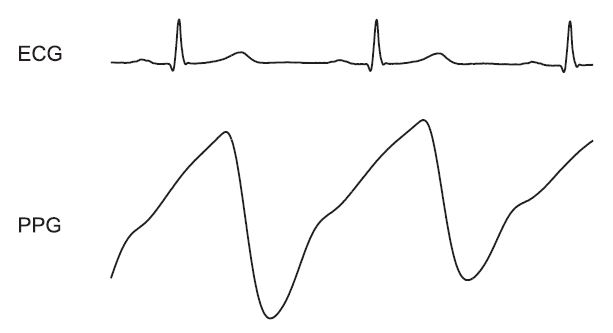
\includegraphics[width=0.7\textwidth, angle=0]{images/ppg_raw.jpg}
	\caption[PPG signal]{The PPG signal and the corresponding ECG. Displayed are the pulsatile AC component, which is super imposed on the much larger DC component. The PPG waveform represents light attenuation in relation to the blood volume in the tissue.}
	\label{ppg_pw}
\end{figure}

Its synchronization with the heart beat makes the AC pulse of the PPG waveform a valuable source of information on heart functions and condition. Based on the appearance of the AC pulse, two phases have been defined, reflecting its two most important properties. The first was labeled as the anacrotic phase and describes the rising edge of the pulse. This part of the waveform is primarily related to the systole. The second phase, shows the effects of diastole and wave reflections from the periphery of the vascular system. This phase is called catacrotic and can be observed in the successive falling edge of the pulse. In healthy subjects there usually is an observable dicrotic notch during this phase.
%[insert: ppg_pw.jpg, source: \cite{Allan2007}]
\begin{figure}[ht]
	\centering
  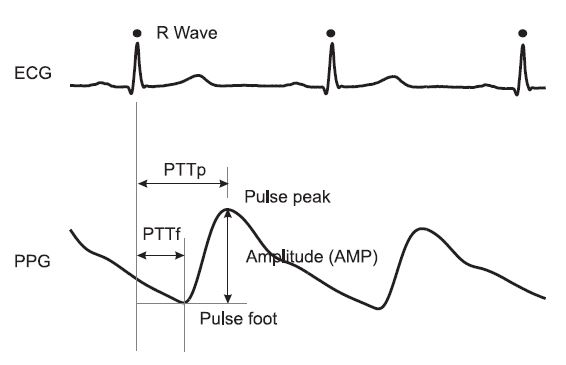
\includegraphics[width=0.7\textwidth, angle=0]{images/ppg_pw.jpg}
	\caption[PPG pulse characteristics]{Characteristics of the PPG pulse waveform in relation to the ECG.}
	\label{ppg_pw}
\end{figure}

In addition to this coarse classification, a number of key landmarks have been defined to facilitate the analysis of the waveform and the underlying physiology. Depicted in \ref{ppg_pw} are the three main features that are derived from a single pulse. The pulse transit time to the foot (\gls{pttf}), and the pulse transit time to the peak (\gls{pttp}) are defined as the time delays between a heartbeat, indicated by the R-wave of the \gls{ecg}, to the onset and the peak of the subsequent AC pulse.
The amplitude of a pulse is determined by the absolute value of the displacement between its base and its peak, which are marked by the aforementioned temporal features.\\
However, the scale of these characteristics, as well as the overall appearance of the waveform are still subject to change. It is believed that these changes are largely caused by reflection of the pulse wave and the tapering down of the arteries towards the periphery \cite{Allan2007}.\\
Another important consideration in the analysis of PPG signals is their susceptibility to movement related artifacts. Although, there are a number of different artifacts that could occur we will only inspect the ones relative to our application. As we employed the Empatica E4, a wrist worn device, to measure \gls{bvp} most of the artifacts are related to large movement of the arm and the wrist but also to small tremors in the hand or fingers. Additionally, extremes in physiological variation such as coughing and marked changes in the breathing pattern prove to be quite influential. Figure \ref{ppg_a} shows an illustration by Allan (2007) depicting the effects of movement related artifacts to one minute PPG recordings that were taken at the index finger.\\

%[insert: ppg_a.jpg, source: \cite{Allan2007}]
\begin{figure}[ht]
	\centering
  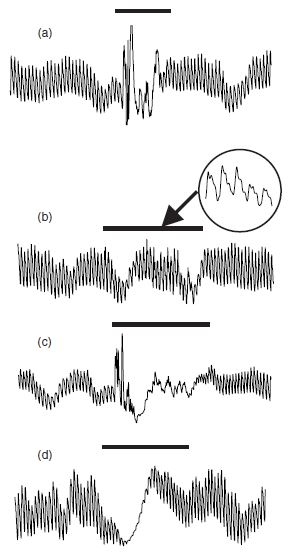
\includegraphics[width=0.5\textwidth, angle=0]{images/ppg_a.jpg}
	\caption[Types of measurement artifacts]{Examples of different types of measurement artifacts. All events were marked by black bars. (a) An episode of gross movement artifact of PPG probe cable tugging. (b) Hand or finger tremor. (c) a bout of coughing, and (d) marked changes in the breathing pattern (a deep gasp or yawn) }
	\label{ppg_a}
\end{figure}

This concludes the section on the general waveform morphology and the reasoning for its variations. Lastly, we will take a closer look at the features we derived from the PPG measurement, specifically heart rate, and heart rate variability.

\subsection{Heart Rate Variability}
Variations in the length of the intervals between consecutive heart beats are called heart rate variability (\gls{hrv}). Typically these inter beat intervals (\gls{ibi}s) are determined by calculating the distance between two subsequent R-peaks of an ECG signal. However, they can also be derived from PPG signals. Again, \gls{ibi}s are the time periods between the maxima of subsequent AC pulses. Since its first appreciation in 1965 HRV experienced a significant increase in popularity due to the apparent ease of derivation from widespread measures, such as ECG and PPG. In 1981, Akselrod et al. introduced power spectral analysis of HRV, contributing to the understanding of its autonomic background by relating the power content of certain frequency bands to sympathetic and parasympathetic activity \cite{TheEuropeanSocietyofCardiology1996}.
In more recent years the increased interest in the application of psychophysiological measures in the field of adaptive automation led to an extensive discussion on HRV as a candidate measure. Byrne et al. (1996) argued in support of HRV as a possible index for both cognitive effort and compensatory effort. But, they also warned against the negligence of situation-related influences (e.g. the given task environment) in the process of signal interpretation. Thereby, a careless approach could have considerable consequences on the efficacy of adaptive automation.\\
In addition, the significance and meaning of the many different HRV measures are more complex than generally appreciated and consequently there is a high potential for incorrect conclusions and for excessive or unfounded extrapolation \cite{TheEuropeanSocietyofCardiology1996}.
In 1996, the European Society of Cardiology and the North American Society of Pacing and Electrophysiology put together a Task Force to address these problem by developing appropriate standards for the acquisition and analysis of HRV.
These standards remain valid until today and help preserving the integrity of HRV analysis if applied correctly.\\
Measures of the HRV can be divided into three general groups, the time domain methods, the frequency domain methods and non-linear methods.

\section{Machine Learning}
Machine learning is a scientific study revolving around the development of algorithms and statistical models that provide computer systems with the ability to automatically learn and improve without being explicitly programmed. Machine learning techniques are commonly categorized as either supervised or unsupervised. This distinction is based on the type of input and output data they use as well as the type of problem they are intended to solve. Supervised learning algorithms require a set of data that contains both the inputs and the desired outputs to a certain problem. Based on this data, often referred to as training data, supervised algorithms derive a function that can be used to predict the output associated with new inputs. Supervised learning algorithms are generally used to solve classification and regression tasks. In contrast unsupervised learning algorithms are able to function on datasets that do not provide any output at all. They attempt to find a structure in the training data, by identifying commonalities. Based on the absence or presence of these similarities in new data they are then able to make predictions. 
Over the years a variety of algorithms have been developed for either category, each with its own objectives, strengths and weaknesses. Identifying an algorithm that is suitable for the desired task is one of the key components to a successful application of machine learning. Therefore, we will now take a closer look at the algorithm selection process used in the recent work. 
  
\subsection{Algorithm Selection}
In the first step of the selection process we considered the work of previous researchers. In particular Wu et al. (2008), who presented the top 10 algorithms identified by the IEEE International Conference on Data Mining (ICDM) in December 2006 \cite{Wu2008}. The algorithms were chosen according to the following steps. First they invited renowned researches of the field to each nominate up to 10 best-known algorithms in data mining. Each nomination had to provide the following information: the algorithm name, a brief justification, and a representative publication reference. After the nominations had been verified, those with less than 50 citations were removed. The remaining nomination were then organized in 10 topics: association analysis, classification, clustering, statistical learning, bagging and boosting, sequential patterns, integrated mining, rough sets, link mining, and graph mining. The final 18 candidates were then put to another vote with a much larger involvement of the research community. The results of this vote were the presented as the top 10 algorithms.\\
From this initial pool of algorithms we then selected those that were assigned to the topic of classification. As Python was the programming language we had agreed upon for all of our machine learning applications. We selected the algorithms that showed the highest compliance with the standard Python libraries from the subset of classification algorithms.  
In the following subsections we will provide a brief description to each of the final four machine learning algorithms.

\subsection{k-NN Classifier}
\subsection{Support Vector Machine}
\subsection{Decision Trees}
scikit-learn uses an optimised version of the CART algorithm; however, scikit-learn implementation does not support categorical variables for now.(https://scikit-learn.org/stable/modules/tree.html)

CART (Classification and Regression Trees) is very similar to C4.5, but it differs in that it supports numerical target variables (regression) and does not compute rule sets. CART constructs binary trees using the feature and threshold that yield the largest information gain at each node.
\subsection{Multi Layer Perceptron}




%\section{Motivation}
%Physical illness, distress, and injury are all well known to be possible consequences of a stressful workplace. 
%Therefore, stress management not only has become a key component in today's industry, but also a common research topic in recent years. Where disciplines such as organizational psychology attempt to address this matter by offering practical guidelines for the assessment and mitigation of workplace stressors, neuroergonomics merges the disciplines of neuroscience and ergonomics to provide for a deeper understanding of the neural bases of perceptual and cognitive functions in relation to technologies and settings in the real world. 
%We take a neuroergonomic approach which attempts to optimize stress management in collaborative workplaces by regulating the information flow of a human-robot-interface (\gls{hri}) according to changes in the mental state of the user. 
%Using a commercial wrist worn device in combination with a processing unit, we designed a  system that is capable of obtaining and interpreting psychophysiologic information in real-time.
%We believe that such a system could not only be a potent tool in risk management, greatly reducing stress related incidents at collaborative workplaces, but also improve overall operating performance.

%In this chapter we will start by giving a brief introduction to the field of automation. Discussing various forms, their benefits, as well as possible downsides. Then we will take a closer look at neuroergonomics and why it could be a crucial adaption to automated systems. Finally we will address stress in the context of human emotions and focus on its connection to the psychophysiologic measures that were used in the scope of this thesis.
%
%\subsection{Automation}
%Automation, in one form or another, has been a dominating force in almost every branch of industry for what has been the better part of two centuries now. It can be defined as the creation and application of technology by which the production and delivery of various goods and services is controlled and monitored with minimal human assistance. 
%Automation can be encountered in many different forms, from a simple control loop in a hydraulic system up to an artificial intelligence handling emergency breaking in cars, based on scans of the surroundings.\\[10pt]
%\textbf{Static automation}\\[10pt]
%Static automation is the traditional form of automation. In this form, automation is an all-or-none technology either performing a task for us or not \cite{Byrne2006}. 
%Although, this brings numerous benefits, such as relieving workers from the strain of performing repetitive tasks, there is increasing evidence that static automation comes at the price of impaired decision making, manual skill degradation, loss of situational awareness, and monitoring inefficiency \cite{Byrne2006}. 
%Introducing static automation into a work environment causes a significant change in roles. 
%This means that workers, once active operators of machines and technology, become passive monitors. In their new position workers often face monitoring workloads that are inherently different and often significantly higher than the manual control conditions of a non automated work environment. In addition to this, the safety of most automated systems is relying heavily on the operators ability to adapt and to achieve their monitoring goals.  
%%All these problems could be linked to the shift in the quality and the quantity of the mental workload, that is caused by static automation. 
%%Further the change in the quality and the quantity of the mental workload, caused by automation, could also be the reason for behavioral adaption, inappropriate trust as well as decreasing job satisfaction. 
%Studies by Parasuraman et al. (1993,1994) tested subjects in a multi-task flight simulator with optionally automatable components and reported a substantial decrease of human operator detection of automation failures after short periods of time in a static automation scenario with constant task assignment of both operator and the automated system \cite{Byrne2006}.
%%Considering these results the negative influences of long-term static automation on system performance become apparent.\\
%These results reflect the negative effects the careless application of long-term static automation could spell on both system performance and operator safety.\\[10pt]
%\textbf{Adaptive automation}\\[10pt]
%Adaptive automation is a concept that has been proposed to resolve the problems of long-term static automation. Whereas static automation is considered to be an agent working for the operator, adaptive automation is viewed as an interactive aid working with the operator \cite{Byrne2006}. It attempts to optimize system performance by adjusting the task assignment between the human operator and automation dynamically. This task reallocation is based on task demands, user capabilities, and system requirements. Another advantage of adaptive over static automation is the ability to reconstruct the task environment in terms of what is automated, how it is automated, what tasks may be shared, and when changes occur \cite{Byrne2006}. However, for these possible regulations to be efficient we require both the operator and the automated system to have sufficient knowledge of each other's current capabilities, performance and state \cite{Byrne2006}.
%As discussed by Byrne et al. (2006), there are three main approaches to address this issue, which either use model-based prediction or continuous measurements to determine the operators current state. In the scope of this thesis we will focus on the latter.
%In conclusion, adaptive automation provides a significant advantage over static automation. Due to the fact that operator capability is emphasized in the process of maximizing system performance, we see a reduction in monitoring efficiency and an incline job satisfaction levels.

\section{Acknowledgments}

